\documentclass{article}
 \usepackage{graphicx}
 \usepackage{subcaption}
 
 \title{Separable and Entangled}
 \date{15-05-2020}
 \author{Bavana Varun Satya Raj}
 \begin{document}
  \maketitle
  \section*{Theory}
  Consider the state $|\psi>=\frac{|00>+|11>+p(|01>+|10>)}{\sqrt{2+2p^2}}$,\\              	Here, when p=0 we have the Bell State $|\psi>=\frac{|00>+|11>}{\sqrt{2}}$  	\\and when p=1, we have $|\psi>=\frac{|00>+|11>+(|01>+|10>)}{2}$,
  	which in turn is\\ $|\psi>=\frac{|0>+|1>)}{\sqrt{2}}\otimes\frac{|0>+|1>)}{\sqrt{2}}$, this is a separable state.\\\\
  	Hence as we increase p from 0 to 1, we go from a maximally 				entangled state to a separable state.
  
  \section*{Code}  
  \subsection*{Importing Required Modules}  
   1. First we import the necessary packages:\\
   2. Numpy enables us to do Tensor product, Matrix multiplication etc\\
   3. scipy stats ortho group imports orthonormal vectors\\
   4. matplotlib.pyplot enables us to plot graphs   

  \subsubsection*{Logic}
   runge=np.arange(0,1,0.01):\\ creates an array runge with values 			ranging from 0 to 1 with step size 0.01.(This Runge is our p)\\\\
   sx=np.array([[0,1],[1,0]])\\
   sy=np.array([[0,-1j],[1j,0]])\\
   sz=np.array([[1,0],[0,-1]])\\
   The above are my Pauli Spin Matrices $\sigma_x$,$\sigma_y$,$\sigma_z$, 	respetively\\\\
   $x=orthogroup.rvs(3)\\
   y=orthogroup.rvs(3)$\\
   The above assigns to x and y orthonormal matrices\\\\
  \begin{displaymath}   
   a1=x[0], 
   a2=x[1], 
   a3=x[2], 
   b1=y[0], 
   b2=y[1], 
   b3=y[2],  
   x^2
  \end{displaymath}
  Assigning each row of x(y) to a1,a2,a3 to get three orthonormal 			vectors.\\\\
  psi=np.array([1,p,p,1])\\
  psi=psi/(np.linalg.norm(psi))\\
  Assigning our state and normalizing it.\\\\
  $    
   def d(a,b):\\
            s1=a[0]*sx+a[1]*sy+a[2]*sz\\
            s2=b[0]*sx+b[1]*sy+b[2]*sz\\
            s=np.kron(s1,s2)\\
            temp=np.matmul(psi,np.matmul(s,psi))$\\
            return temp\\
  Here 's1' and 's2' each represent $\sigma$.$\bar{a}$ and $\sigma$.$                      	\bar{b}$ respectively
  's' is the Tensor product of s1 and s2.\\
  'temp' is the expectation value.\\\\
     
  What we do later is, for each value of 'p' we find the maximum CHSH 			value for 100000 times(each time the orthonormal triads being 			different) and take mean of all those thousand maxima.\\
  Hence, for each p we have the average of maxima taken 100000 times
  and plot the results
  \clearpage
 \begin{figure}[b!]
  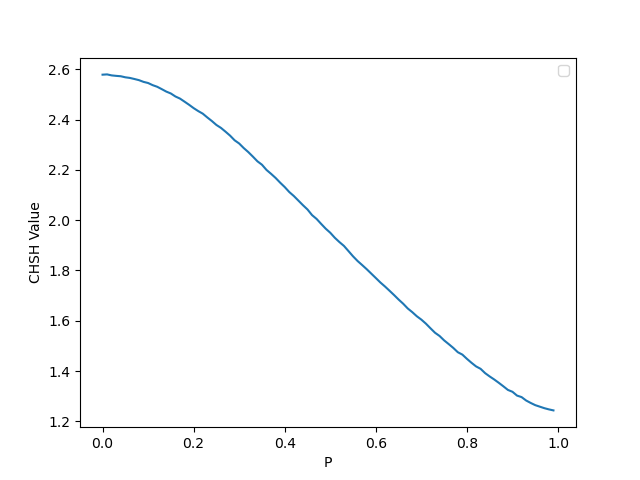
\includegraphics[width=\linewidth]{better.png}
  \caption*{Numerical Result}
  \label*{}
 \end{figure}
 \end{document}